\documentclass[11pt,english,letterpaper,oneside]{article}
\usepackage{amsmath,amssymb,amsfonts,amsthm,enumerate,enumitem}
\usepackage[top=3cm,bottom=3cm,left=2.5cm,right=2.5cm]{geometry}
\usepackage{graphicx,microtype}
\usepackage[T1]{fontenc}
\DisableLigatures[f]{encoding=T1}
\usepackage[skip=2pt]{caption}
\usepackage{subcaption}
\usepackage{hyperref,lineno}
\linenumbers
\usepackage{textcomp}
\usepackage{setspace,array,float}
\usepackage{bm}
\usepackage{rotating}
\usepackage{hhline}
\usepackage{color}
\usepackage{delarray}
\usepackage[compact]{titlesec}
\usepackage[none]{hyphenat}
\setlength{\parskip}{0cm}
\usepackage{natbib}
\setcitestyle{citesep={;},aysep={}}
\usepackage{babel}
\pagestyle{plain}
\frenchspacing
\doublespacing
\usepackage{sectsty}
\usepackage[table]{xcolor}
\allsectionsfont{\bfseries}


%%%%%%%%%%%%%%%%%%%%%%%%%%%%%%%%%%%%%%%%%%%%%%%%%

\begin{document}

\newcommand{\tmat}{$\bm{T}$}
\newcommand{\rmat}{$\bm{R}$}

\vspace*{0.25in}

\begin{center}

{\Large \textbf{Estimating allele frequencies in non-model polyploids using high throughput sequencing data}}
\vspace{0.45in}

Paul D. Blischak,$^{1,\dagger}$ Laura S. Kubatko$^{1,2}$ and Andrea D. Wolfe$^1$
\vspace{0.45in}


\textit{$^1$Department of Evolution, Ecology and Organismal Biology, The Ohio State University,}

\textit{318 W. 12th Avenue, Columbus, OH 43210, USA.}
\bigskip
\bigskip

\textit{$^2$Department of Statistics, The Ohio State University,}

\textit{1958 Neil Avenue, Columbus, OH 43210, USA.}


\end{center}
\vspace{0.45in}


\noindent $^\dagger$\textbf{Corresponding author}: Paul Blischak, Dept. of Evolution, Ecology and Organismal Biology, Aronoff Laboratory, The Ohio State University, 318 W. 12th Avenue, Columbus, OH 43210. E-mail: blischak.4@osu.edu.
\vspace{0.45in}

\noindent \textbf{Keywords}: polyploidy, population genomics, hierarchical Bayesian modeling, RAD sequencing, \textsc{polyfreqs}
\vspace{0.45in}

\noindent \textbf{Running title}: Allele frequencies in polyploids

\vfill

%%%%%%%%%%%%%%%%%%%%
\section*{Abstract}                      %%
%%%%%%%%%%%%%%%%%%%%

Despite the ever increasing opportunity to collect large-scale datasets for population genomic analyses, the use of high throughput sequencing to study populations of polyploids has seen little application. This is due in large part to problems associated with determining allele copy number in the genotypes of polyploid individuals (allelic dosage uncertainty--ADU), which complicates the calculation of important quantities such as allele frequencies. This well known problem has hindered population genetic studies in polyploids for decades, though several tools exist for analyzing genetic data from polyploids by dealing with particular issues of ADU. Additional complications arise because of the mixed inheritance patterns and variable reproductive modes that are characteristic of many polyploid taxa, making the development of population genetic models for polyploids especially difficult. Here we describe a statistical model to estimate biallelic SNP frequencies in a population of polyploids using high throughput sequencing data in the form of read counts. Uncertainty in the number of copies of an allele in an individual's genotype is accounted for by treating genotypes as an intermediate parameter in a hierarchical Bayesian model. In this way, we bridge the gap from data collection (using techniques such as restriction-site associated DNA sequencing) to allele frequency estimation in a unified inferential framework by summing over genotype uncertainty. Simulated datasets were generated under various conditions for both tetraploid and hexaploid populations to evaluate the model's performance and to help guide the collection of empirical data. We also discuss potential sources of bias that could influence results, as well as propose model extensions to ameliorate some of these biases.
\medskip

%%%%%%%%%%%%%%%%%%%
\section*{Introduction}            %%
%%%%%%%%%%%%%%%%%%%

\textbf{Paragraph 1: The importance of polyploidy}---The process of whole genome duplication (WGD) has come to be acknowledged as an important evolutionary force in the generation of potentially adaptive genetic variation \citep{otto2000polyploidy,soltis2000PNASployploidy,soltisD2003polyploid,soltisd2009diversification,soltisd2010polyploidUnknowns,soltisd2014stebbins,Selmecki2015yeastAdaptation}. Though its effects were initially debated \citep{wagner1970noise,StebbinsVariationEvolution}, a reevaluation of the prevalence and impact of WGD has solidified its influence at evolutionary time scales both deep and shallow \citep{soltisd2004tragopogon,comai2005polyploid,cui2006genomeDuplication,jiao2011ancientWGD,canon2014polyploidyLegumes,douglas2015diploidizationCapsella}. 
\medskip

\textbf{Paragraph 2: The history of models for polyploids}---The theoretical treatment of population genetics models in polyploids has it origins in the Modern Synthesis, with  Fisher, Haldane and Wright each contributing to the development of some of the earliest mathematical models for understanding allele frequencies in polyploids \citep{haldane1930autopolyploids,wright1938polyploid,}. Among the earliest of these papers was Haldane's extension of the Hardy-Weinberg theorem to arbitrary ploidy, as well as his treatment of autotetraploid inhertance. Fisher's interest in polyploidy stemmed largely from observations made in the plant genus , which exhibited differing levels of heterostyly. The further observation of mixed ploidy-levels within the populations led Fisher to examine patterns of inheritance of polyploids. Wright's contributions were concerned mostly with the calculation of changes in allele frequencies through mutation, migration and to some degree selection, and can be considered a simple extension of his previous work on allele frequencies to the case of a $2k$-ploid. \cite{moody1993autopolyploids} It was also noted by Moto Kimura in his papers on diffusion processes for allele frequencies that models such as Wright's $\phi$ could potentially be applied to polyploid organisms \citep{kimura1964diffusion}. All of these models depend on the accurate estimation of genotypes, which has been the Achilles' heel of polyploid population genetics. For a more contemporary review on population genetics in polyploids see \cite{dufresne2014polyPopGen} and references within.
\medskip

\textbf{Paragraph 3: Brief overview of model for polyploids and high throughput sequencing}---There are few examples of RADseq experiments (but see \citep{logan-young2015polyploidSNP}).
\medskip

\textbf{Paragraph 4: Explain what the model here accomplishes}---The model described here aims to tackle problems associated with allelic dosage uncertainty.
\medskip

%%%%%%%%%%%%%%%%%%%%%%%%%%%
\section*{Materials and methods}                  %%
%%%%%%%%%%%%%%%%%%%%%%%%%%%

\noindent Our aim is to estimate the frequency of a reference allele for each locus sampled from a population of known ploidy, where the reference allele can be chosen arbitrarily between the two alleles at a given SNP. To do this we extend the population genomic models of \cite{buerkle2013popModels}, which employ a Bayesian framework to model next-generation sequencing reads, genotypes and allele frequencies, to the case of arbitrary ploidy. The basic idea is to view the sequencing reads gathered for an individual as a random sample from the unobserved genotype at a given locus. Genotypes can then be used as a parameter in a probability model that governs how likely it is that we see a particular number of sequencing reads carrying the reference allele. Similarly, we can treat genotypes as a random sample from the underlying allele frequency in the population (assuming Hardy-Weinberg equilibrium). This hierarchical setup addresses the problems associated with ADU by treating genotypes as a nuisance parameter that we integrate out using Markov chain Monte Carlo (MCMC). . Figure \ref{fig1} gives an illustration of the model for a tetraploid ($\psi=4$) and Table \ref{table1} provides a reference for the notation and symbols used in the description of the model below.

\medskip
\subsection*{Model setup}
\medskip

Here we consider a sample of $N$ individuals from a single population of ploidy-level $\psi\: (\psi\geq2)$ sequenced at $L$ unlinked SNPs. The data for the model consist of two matrices containing counts of reads typically generated by high throughput sequencing platforms: \tmat{} and \rmat. The $N\times L$ matrix \tmat{} contains the total number of reads sampled at each locus for each individual. Similarly, \rmat{} is an $N\times L$ matrix containing the number of sampled reads with the chosen reference allele at each locus for each individual. Assuming conditional independence of the sequencing reads given genotypes the probability distribution for sequencing reads can be factored

\begin{equation}\label{factored_lik}
P(\bm{R}|\bm{T},\bm{G}) = \displaystyle\prod_{\ell=1}^L\displaystyle\prod_{i=1}^N P(r_{i \ell}|t_{i \ell},g_{i \ell})
\end{equation}

\noindent For an individual, $i$, at a particular locus, $\ell$, we model the number of sequencing reads containing the reference allele ($r_{i\ell}$) as a Binomial random variable conditional on the total number of sequencing reads ($t_{i\ell} $), the underlying genotype ($g_{i\ell}$) and a constant level of sequencing error ($\epsilon$)

\begin{equation}\label{likelihood}
{P}(r_{i \ell}|t_{i\ell}, g_{i \ell},\epsilon) = \binom{t_{i \ell}}{r_{i \ell}}
	\begin{cases}
	\epsilon^{r_{i \ell}}(1-\epsilon)^{t_{i \ell}-r_{i \ell}} & \text{if  } g_{i \ell} = 0, \\[0.05in]
	\left(\frac{g_{i \ell}}{\psi}\right)^{r_{i \ell}}\left(1-\frac{g_{i \ell}}{\psi}\right)^{t_{i \ell}-r_{i \ell}} & \text{if  } g_{i \ell} = 1,\ldots,\psi-1, \\[0.05in]
	(1-\epsilon)^{r_{i \ell}}\epsilon^{t_{i \ell}-r_{i \ell}} & \text{if  } g_{i \ell} = \psi\,.
	\end{cases}
\end{equation}


\noindent Since the $r_{i \ell}$'s are the data that we observe, the product of $P(r_{i \ell}|t_{i\ell}, g_{i \ell},\epsilon)$ across loci and individuals will form the likelihood in the model. An important consideration here is that when $g_{i \ell}$ is equal to 0 or $\psi$ (i.e., when the genotype is homozygous) the likelihood will always be 0. To correct for this, we include error ($\epsilon$) into the model. The intuition behind including error is that we may have just not sampled the alternative allele due to lack of sequencing depth or due to a sequencing error. When we do this, the probability distribution for $r_{i\ell}$ given $g_{i\ell}$ and $\epsilon$ is split into $\psi+1$ cases as above in Eq. \ref{likelihood}.


The model for genotypes will also be Binomial with parameter

\begin{equation}\label{condl_prior}
P(\bm{G}|\psi, \bm{p}) = \displaystyle\prod_{\ell=1}^L\displaystyle\prod_{i=1}^N P(g_{i \ell}|\psi, p_{\ell})
\end{equation}

The joint posterior distribution of allele frequencies and genotypes is equal to the product across all loci and all individuals of the likelihood, the conditional prior on genotypes and the prior distribution on allele frequencies up to a constant of proportionality

\begin{equation}\label{posterior}
{P}(\,\bm{p},\bm{G}|\bm{R},\epsilon) \propto \displaystyle\prod_{\ell=1}^L\displaystyle\prod_{i=1}^N {P}(r_{i \ell}|t_{i\ell}, g_{i \ell},\epsilon){P}(g_{i \ell}|\psi, p_{\ell}){P}(p_{\ell})\,.
\end{equation}

\noindent The marginal posterior distribution for allele frequencies can then be obtained by summing over genotypes

\begin{equation}\label{marg_post_p}
{P}(\,\bm{p}|\bm{R},\epsilon) \propto \displaystyle\sum_{\bm{G}} {P}(\,\bm{p},\bm{G}|\bm{R},\epsilon)\,.
\end{equation}

\noindent It would also be possible to examine the marginal posterior distribution of genotypes but here we focus on allele frequencies only.

\medskip
\subsection*{Full conditionals and MCMC using Gibbs sampling}
\medskip

\noindent We estimate the joint posterior distribution for allele frequencies and genotypes in Eq. \ref{posterior} using Markov chain Monte Carlo (MCMC). This is done using Gibbs sampling of the states $(\,\bm{p},\bm{G})$ in a Markov chain by alternating samples from the full conditional distributions of $\bm{p}$ and $\bm{G}$. Given the setup for our model using Binomial and Beta distributions (which form a conjugate family), analytical solutions for these distributions can be readily acquired \citep{gelman2014bayesian}. The full conditional distribution for allele frequencies is Beta distributed and is given by Eq. \ref{p-full} below:

\begin{equation}\label{p-full}
{P}(\,p_{\ell}|g_{i \ell},r_{i \ell},\epsilon) = \text{Beta}\left(\alpha= \sum_{i=1}^N g_{i \ell} +1,\; \beta = \sum_{i=1}^N (\psi-g_{i \ell})+1\right),\quad \text{for } \ell = 1,\ldots,L.
\end{equation}

\noindent This full conditional distribution for $p$ has a natural interpretation as it is roughly centered at the proportion of sampled alleles carrying the reference allele divided by the total number of alleles sampled $\frac{\alpha}{\alpha+\beta}$. The ``$+1$'' comes from the prior distribution and won't have a strong influence on the posterior distribution when the sample size is large.

The full conditional distribution for genotypes is split into $\psi+1$ cases (similar to the conditional prior), making it a discrete categorical distribution over the possible values for the genotypes $(0,\ldots,\psi)$. Using $k$ as a generic index, the distribution for individual $i$ at locus $\ell$ is

\begin{equation}\label{G-full}
{P}(g_{i \ell}|g_{\text{-}i \ell},p,r_{i \ell},\epsilon) = \frac{1}{\mathcal{C}} \;
	\begin{cases}
	\epsilon^{r_{i \ell}}(1-\epsilon)^{t_{i \ell}-r_{i \ell}}(1-p)^\psi & \text{for  } k = 0, \\[0.05in]
	\left(\frac{k}{\psi}\right)^{r_{i \ell}}\left(1-\frac{k}{\psi}\right)^{t_{i \ell}-r_{i \ell}}\displaystyle\binom{\psi}{k}p^{k}\,(1-p)^{\psi-k} & \text{for  } k = 1,\ldots,\psi-1, \\[0.05in]
	(1-\epsilon)^{r_{i \ell}}\epsilon^{t_{i \ell}-r_{i \ell}}p^\psi & \text{for  } k = \psi\,,
	\end{cases} 
\end{equation}

\noindent where $g_{\text{-}i \ell}$ is the value of the genotypes for all sampled individuals excluding individual $i$ and $\mathcal{C}$ is a normalizing constant equal to the sum of all of the terms:

\begin{equation*}
\mathcal{C} = \epsilon^{r_{i \ell}}(1-\epsilon)^{t_{i \ell}-r_{i \ell}}(1-p)^\psi + (1-\epsilon)^{r_{i \ell}}\epsilon^{t_{i \ell}-r_{i \ell}}p^\psi + \sum_{k=1}^{\psi-1}\left(\left(\frac{k}{\psi}\right)^{r_{i \ell}}\left(1-\frac{k}{\psi}\right)^{t_{i \ell}-r_{i \ell}}\binom{\psi}{k}\,p^k(1-p)^{\psi-k}\right).
\end{equation*}

\medskip
\subsection*{Simulation study}
\medskip

Simulations were performed to assess error rates in allele frequency estimation for tetraploid and hexaploid populations. Data were generated under the model by sampling genotypes from a binomial distribution conditional on a fixed, known allele frequency $(\,p = 0.2, 0.4, 0.6, 0.8)$. Total read counts per individual were simulated for a single locus using a Poisson distribution with mean coverage equal to $\lambda$ $(\lambda = 5, 10, 15, 20)$, followed by the sampling of sequencing reads containing the reference allele from a binomial distribution conditional on the number of total reads, the genotype and sequencing error ($\epsilon$ fixed to 0.01). We varied the number of individuals sampled per population $(N = 5, 10, 20, 30)$ and ran all possible combinations of the simulation settings. Each combination of sequencing coverage, individuals sampled and allele frequency was analyzed using 100 replicates for both tetraploid and hexaploid populations for a total of 12,800 simulation runs. MCMC analyses using Gibbs sampling were run for 500,000 generations with parameter values stored every 500 samples. The first 25\% of the posterior was discarded as burn-in, resulting in 750 posterior samples for each replicate. Convergence on the stationary distribution, $P(\,\bm{p},\bm{G}|\bm{R},\epsilon)$, was assessed by examining trace plots for a subset of runs for each combination of settings and ensuring that the effective sample sizes (ESS) were greater than 200. Deviations from the known underlying allele frequency used to simulate each data set were calculated using the posterior mean of each of the 100 replicates for a given simulation set and comparing it to the known frequency using the root mean squared error (RMSE).
\medskip

All simulations were performed using the R statistical package \citep{r2014} on the Oakley cluster at the Ohio Supercomputer Center (\url{https://osc.edu}). Figures were generated using the R add-on packages \textsc{ggplot2} \citep{wickham2009ggplot2}, \textsc{reshape} \citep{wickham2011plyr} and \textsc{plyr} \citep{wickham2007reshape} with additional figure manipulation completed using Inkscape (\url{https://inkscape.org}). MCMC diagnostics were done using the \textsc{coda} package \citep{plummer2006coda}. Scripts for simulating and analyzing the datasets, as well as for reproducing all figures, are available on GitHub (\url{https://github.com/pblischak/polyfreqs-ms-data}).
\medskip

%%%%%%%%%%%%%%%%%
\section*{Results}               %%
%%%%%%%%%%%%%%%%%

Varying the level of coverage and the number of individuals (Figure \#).
\medskip

It is important to note that we are generating data under the model in the first place, which . However, the high levels of accuracy reported by some of the simulation conditions should not be interpreted as our being selective of settings that show that the model works well, but as validation that the model works when it is supposed to. Analyses of empirical data will obviously not have known values against which the estimated allele frequencies can be compared, but data collection can be informed by these simulations to optimize the number of individuals sequenced per population and the average coverage per locus per individual to obtain good results based on financial resources. Assessments of model adequacy would be also be straightforward to employ to 
\medskip

%%%%%%%%%%%%%%%%%%%
\section*{Discussion}               %%
%%%%%%%%%%%%%%%%%%%

Talk about general discussion points here and maybe include stuff about sources of bias here rather than dedicating an entire section to it.

\medskip
\subsection*{Potential sources of bias}
\medskip

There are two places where bias can be introduced into the estimation of allele frequencies using this model.
\medskip

At the level of read counts, unsampled alleles will obviously bias the resulting
\medskip

Another potential source of bias is treating genotypes among individuals in the population as independent. Polyploid taxa often become apomictic upon genome duplication, and asexual reproduction will generate clonal individuals with identical genotypes. This correlation 

\medskip
\subsection*{Model adequacy}
\medskip

Talk about the adequacy of the model for descrigin biological reality of polyploids. Emphasize the fact that the model directly contributes to ameliorate the issues associated with ADU.

\begin{equation}
P(\tilde{\bm{R}}|\bm{R},\epsilon) = \displaystyle\int \left(\displaystyle\sum_{\bm{G}} P(\tilde{\bm{R}}|\bm{p},\bm{G}) P(\bm{p},\bm{G}|\bm{R},\epsilon)\right) \text{d}\bm{p}\, .
\end{equation}

\medskip
\subsection*{Extensibility}
\medskip

Talk about how the model can serve as a jumping off point for new models that now that ADU may no longer be as much of an issue. Examples are below.
\medskip

Replace $\psi$ with a vector of values representing the ploidy of each individual $(\bm{\psi} = \{\psi_1,\ldots,\psi_N\})$.
\medskip



%%%%%%%%%%%%%%%%%%%%%%%
\section*{Acknowledgements}           %%
%%%%%%%%%%%%%%%%%%%%%%%

The authors would like to thank the Ohio Supercomputer Center for access to computing resources and Nick Skomrock for assistance with deriving the full conditional distributions of the model in the diploid case. This manuscript was also greatly improved by comments from the Associate Editor, \textit{editor name}, and \# anonymous reviewers.
\medskip

%%%%%%%%%%%%%%%%%%%%%%%
\section*{Author Contributions}        %%
%%%%%%%%%%%%%%%%%%%%%%%

Conceived of the study: PDB, LSK and ADW. PDB derived the polyploid model, ran the simulations, coded the R package and wrote the manuscript. PDB, LSK and ADW reviewed all parts of the manuscript and all authors approved of the final version.
\medskip

%%%%%%%%%%%%%%%%%%%%%%
\section*{Data Accessibility}            %%
%%%%%%%%%%%%%%%%%%%%%%

R and bash scripts for simulating the datasets, analyzing them using Gibbs sampling and producing the figures from the resulting output can be all be found on GitHub (\url{https://github.com/pblischak/polyfreqs-ms-data}). We also provide an implementation of the Gibbs sampler for estimating allele frequencies in the R package \textsc{polyfreqs} (\url{https://github.com/pblischak/polyfreqs}). See the package wiki for more details (\url{https://github.com/pblischak/polyfreqs/wiki}).
\vspace{0.5in}

%%%%%%%%%%%%%%%%%
% References                       %%
%%%%%%%%%%%%%%%%%

\singlespacing

\bibliographystyle{molEcol}
\bibliography{references}

\vfill

%%%%%%%%%%
% Tables          %%
%%%%%%%%%%

\begin{table}[b]
\centering
\rowcolors{1}{white}{gray!25}
\caption{Notation and symbols used in the description of the model for estimating allele frequencies in polyploids. Vector and matrix forms of the variables are also provided when appropriate.}
\vspace{0.2in}
\bgroup
\def\arraystretch{1.45}
\begin{tabular}[l]{l | l}
\hline
\textbf{Symbol} & \textbf{Description}\\ \hline
$L$ & The number of loci. \\
$\ell$ & Index for loci ($\ell\; \in \{1,\ldots,L\}$). \\
$N$ & Total number of individuals sequenced. \\
$i$ & Index for individuals ($i\; \in \{1,\ldots,N\}$). \\
$\psi$ & The ploidy-level of individuals in the population (e.g., tetraploid: $\psi$=4). \\
$p_{\ell}$ & Frequency of the reference allele at locus $\ell$. [$\bm{p}$] \\
$g_{i \ell}$ & The number of copies of the reference allele for individual $i$ at locus $\ell$. [$\bm{G}$] \\
$t_{i \ell}$ & The total number of reads for individual $i$ at locus $\ell$. [$\bm{T}$] \\
$r_{i \ell}$ & The number of reads with the reference allele for individual $i$ at locus $\ell$. [$\bm{R}$] \\
$\epsilon$ & Sequencing error. \\
$\lambda$ & Average number of reads sequenced for an individual at a given locus (coverage). \\
\hline
\end{tabular}
\egroup
\label{table1}
\end{table}

%%%%%%%%%%%
% Figures           %%
%%%%%%%%%%%

\begin{figure}[b]
\centering
\caption{The cartoon here illustrates the hierarchical Bayesian model for biallelic SNP frequencies of \cite{buerkle2013popModels}.  Here it is modified for a tetraploid, but can be used for any ploidy level. We will consider the blue allele to be ancestral (as determined by the outgroup, $O$) and red will be the derived allele. The ultimate goal is to approximate the posterior distribution $P(\,p,g|R^b,\epsilon)$, which is the distribution of the frequency of the derived allele in the population at a particular locus and the genotypes at that locus given the number of sequencing reads having the derived allele. The procedure for estimating this distribution is to use Markov chain Monte Carlo methods to draw samples from the posterior distribution of allele frequencies and genotypes given sequencing reads and error. In this example, the genotype ($g$) is drawn from a Binomial(4,$p$), where $p$ is modeled by a Beta(1,1) distribution, and is equal to 3. The likelihood is also given by a binomial distribution with the observed number of successes equal to 10 reads given parameters $n$ equal to 16 total reads and $prob$ equal to $\frac{3}{4}$. The equations in red boxes indicate how one iteration of the sampling would proceed. First a proposed value for p is randomly selected and is modeled by a Beta(1,1). This value for $p$ is then be used as the $prob$ parameter to draw a random genotype from the binomial distribution. This genotype is then divided by the ploidy level to give the value of the $prob$ parameter in the binomial likelihood.}
\vspace{0.5in}
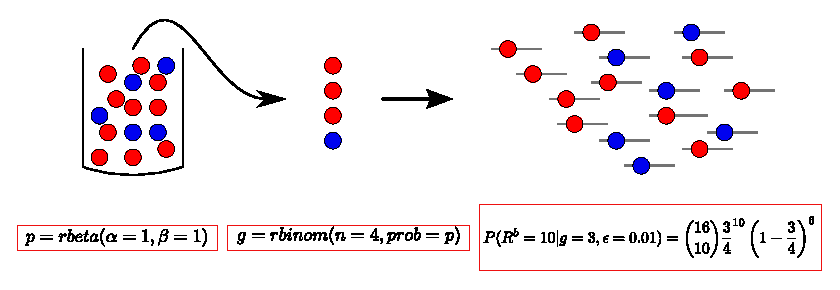
\includegraphics[width=\textwidth]{pop-gen-model}
\smallskip
\label{fig1}
\end{figure}

\begin{figure}[b]
\centering
\caption{Heat maps representing the relative error of the model for estimating allele frequencies across various simulation conditions.}
\vspace{0.5in}
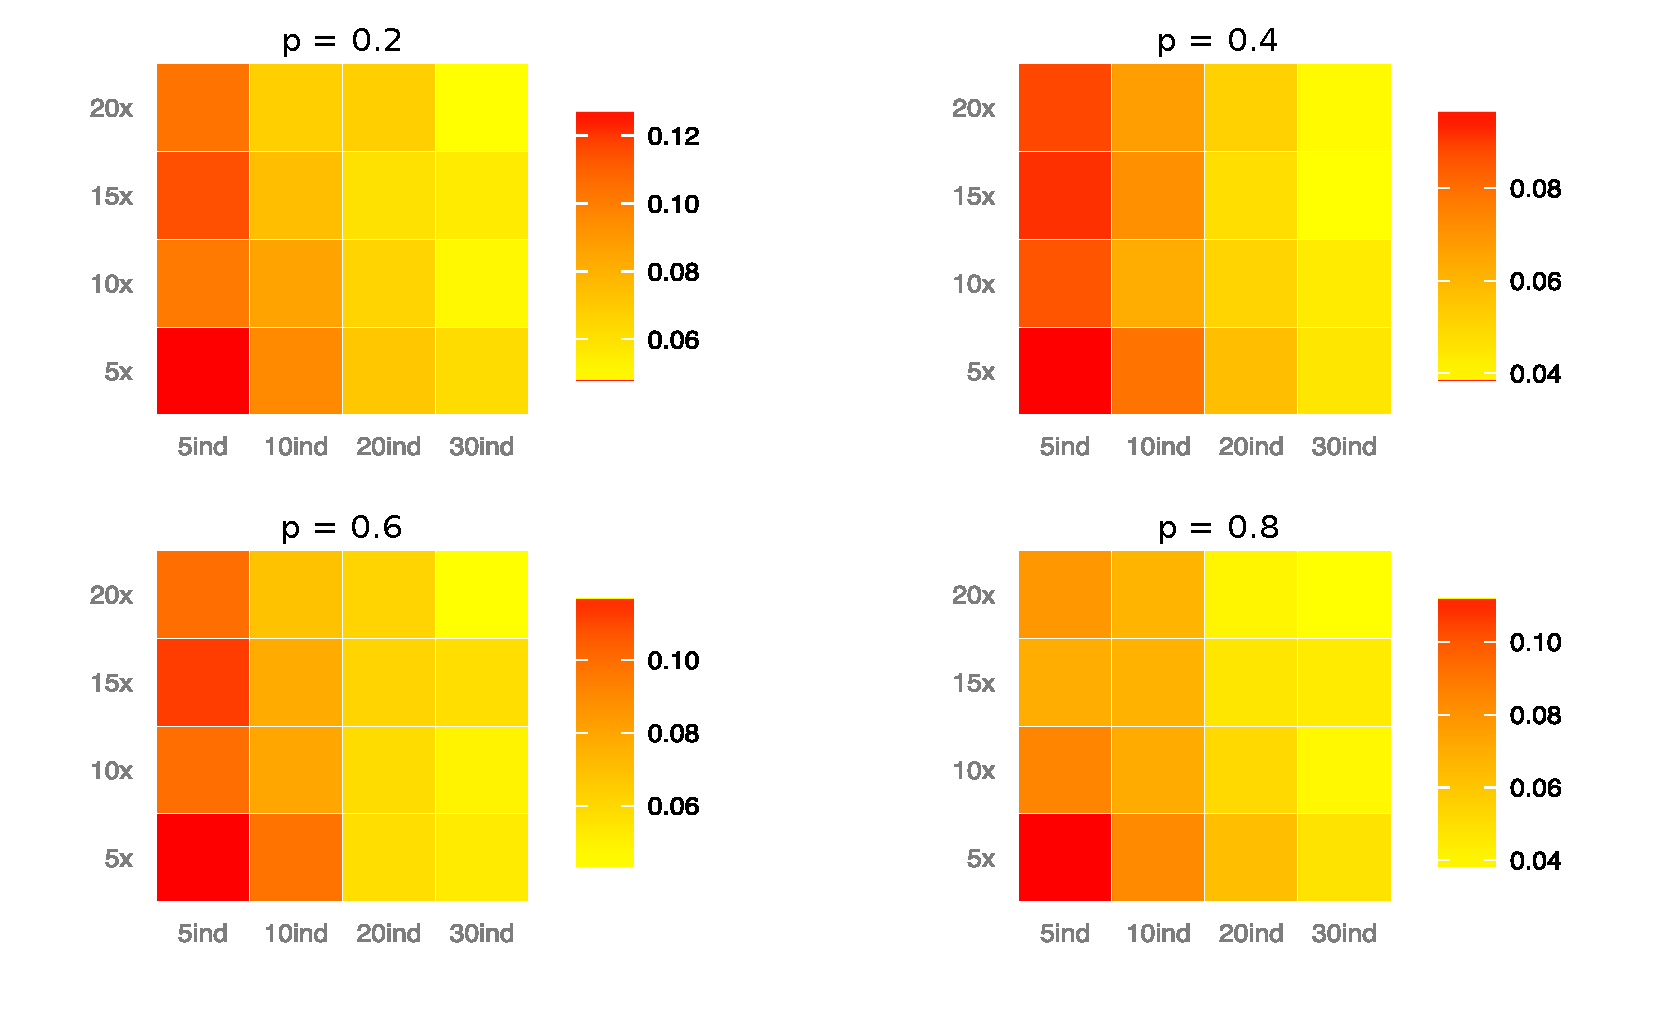
\includegraphics[width=\textwidth]{tetra-heatmaps}
\smallskip
\label{fig2}
\end{figure}

\end{document}